\documentclass{scrartcl}

\usepackage{geometry}
 \geometry{
 a4paper,
 left=3cm,
 right=3cm,
 top=3cm,
 bottom=15mm,
 }
\usepackage[utf8]{inputenc}
\usepackage{amsmath,tikz}
\usepackage{amssymb}
\usepackage{lastpage,enumerate,listings}
\usepackage{fancyhdr}
\usepackage{mathtools}
\usepackage{marvosym}
\usepackage{float}
\usetikzlibrary{shapes,trees,positioning}
\setlength{\headheight}{39		pt}
\DeclarePairedDelimiter{\ceil}{\lceil}{\rceil}
\fancyhead[l]{Praktische Optimierung mit Modellierungssprachen\\[1ex] \textbf{\LARGE Exercise Series 6}}
\fancyhead[c]{\thepage / \pageref{LastPage}}
\fancyhead[r]{ Dominik Chmiel  308611 \\ Marcel Jonda 359684}
\fancyfoot{}
\pagestyle{fancy}

\newcommand{\derive}[2] {\xRightarrow{#1}{}_{\hspace{-3pt} #2}\;}
\usepackage{tikz}
\usetikzlibrary{automata,positioning}
\begin{document}

\begin{figure}
\begin{tabular}{cc}
  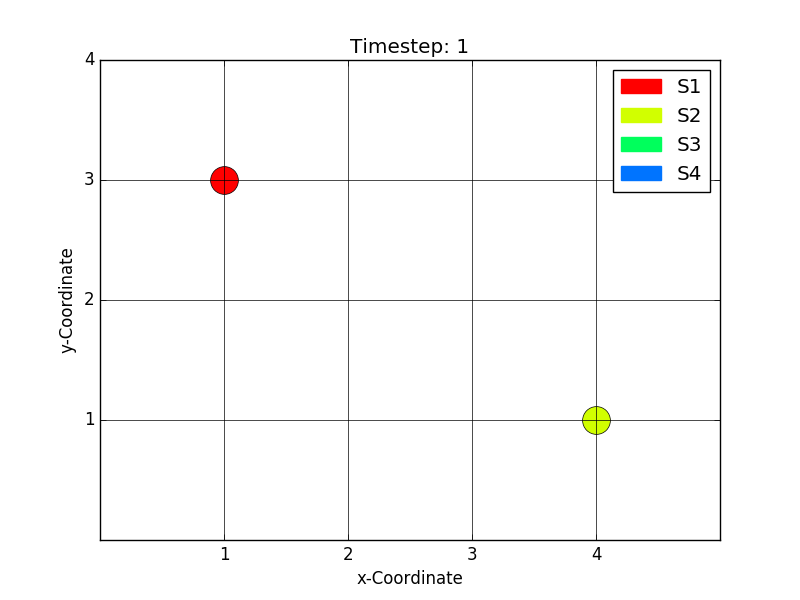
\includegraphics[width=65mm]{routing_t_1.png} &   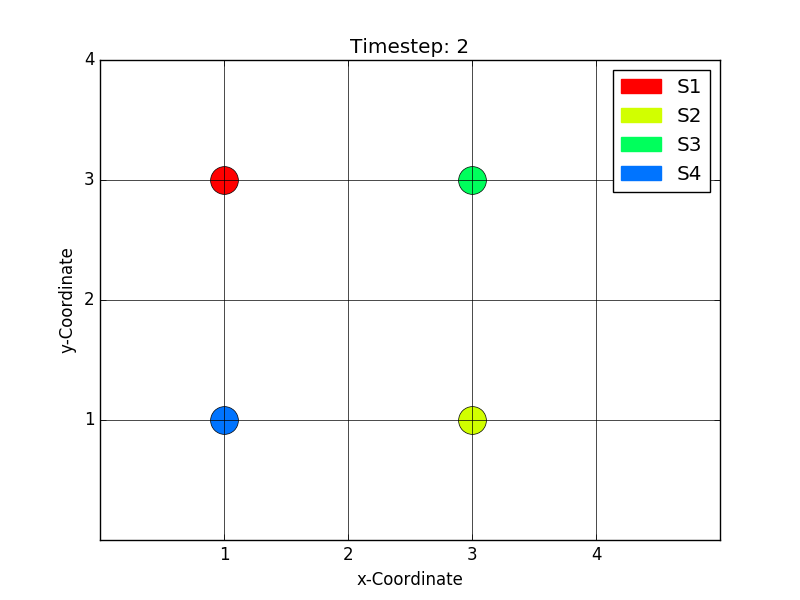
\includegraphics[width=65mm]{routing_t_2.png} \\
Step $t=1$ & Step $t=2$ \\[6pt]
 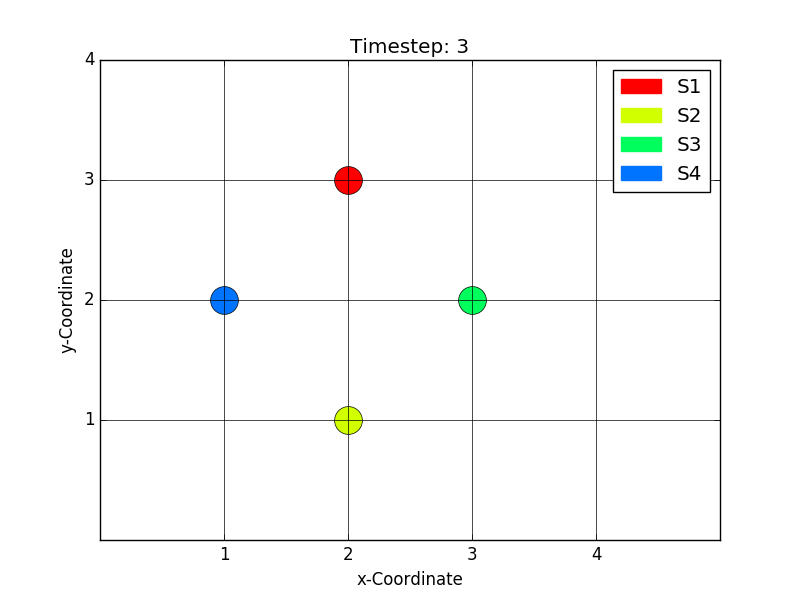
\includegraphics[width=65mm]{routing_t_3.png} &   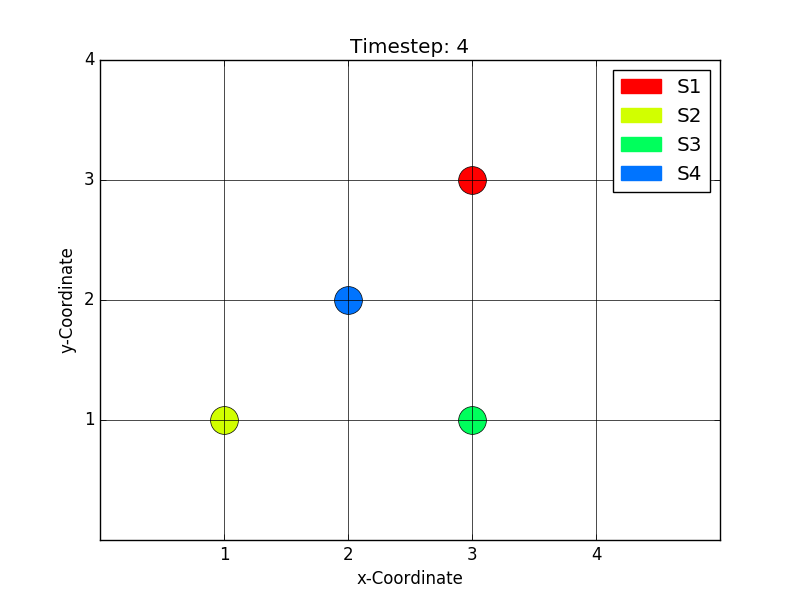
\includegraphics[width=65mm]{routing_t_4.png} \\
Step $t=3$ & Step $t=4$ \\[6pt]
 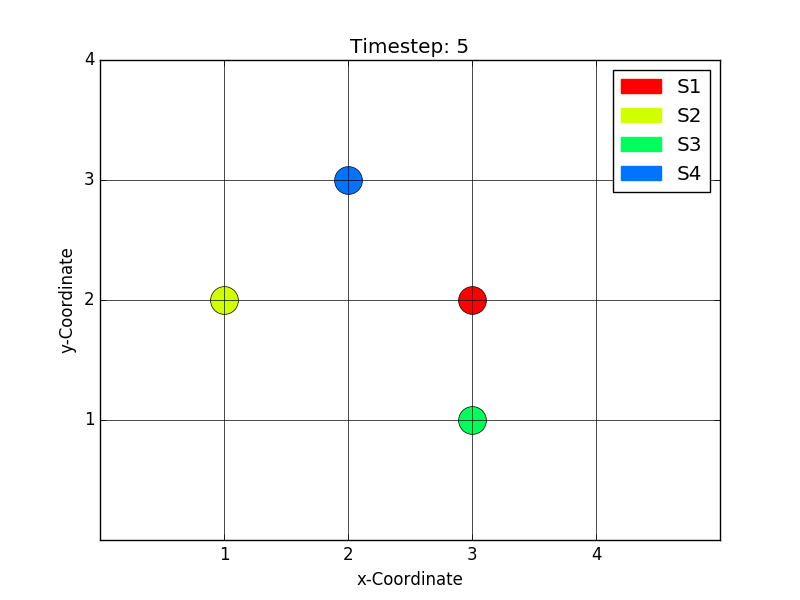
\includegraphics[width=65mm]{routing_t_5.png} &   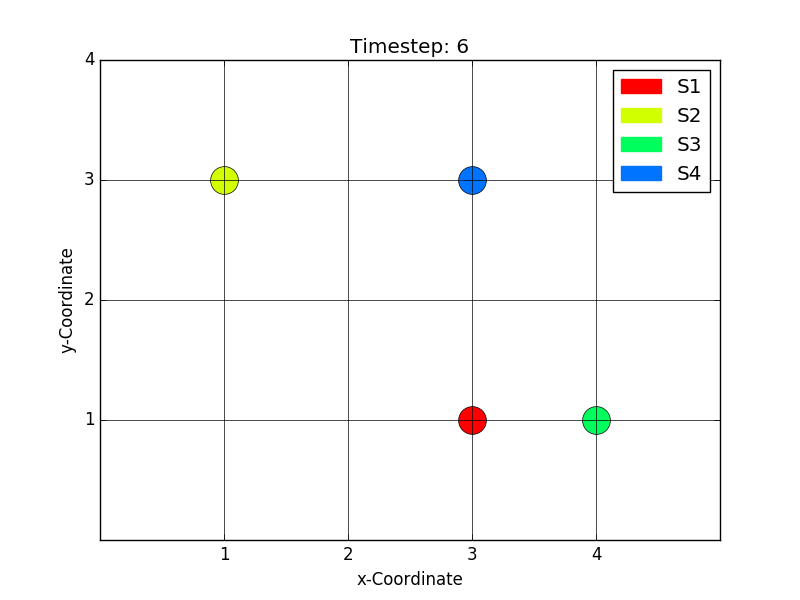
\includegraphics[width=65mm]{routing_t_6.png} \\
Step $t=5$ & Step $t=6$\\[6pt]
\end{tabular}
\caption{Solution of Instance 2}
\end{figure}


\end{document}  